\chapter{Estado del Arte}
\label{chapter:estadoarte}


El objetivo de este apartado es hacer un recorrido por el estado del arte relacionado con el proyecto, este recorrido lo enfocaremos desde tres puntos de vista diferentes:
\begin{itemize}
	\item \textbf{Procesamiento del Lenguaje Natural}: En este apartado nos centraremos en el procesamiento del lenguaje natural y su evolución a lo largo del tiempo. 
	\item \textbf{\textit{Deep Learning} y aplicación al Procesamiento del Lenguaje Natural}: En la segunda parte pondremos foco en el \textit{Deep Learning}, sus ventajas y cómo se están aplicando estos métodos al procesamiento de lenguaje natural. 
	\item \textbf{\textit{Big Data} y \textit{Fast Data}}: Por último, haremos un repaso a la evolución del \textit{Big Data} y cómo la tendencia actual es realizar el procesamiento en tiempo real mediante \textit{Fast Data}.
\end{itemize}

\section{Procesamiento de lenguaje natural}

\subsection{Historia}

Para hablar de los orígenes del procesamiento del lenguaje natural (a partir de ahora NLP por sus siglas en inglés \textit{Natural Lenguage Processing}) tal y como lo conocemos, tendríamos que remontarnos a los años 50, concretamente al artículo ``\textit{Computing Machinery and Intelligence}'' escrito por Alan Turing \cite{turing_1950}. En este artículo aparece el NLP dentro del campo de la inteligencia artificial y se presenta por primera vez el conocido ``Test de Turing`''. Este test convirtió la pregunta abstracta de ``¿Son capaces de pensar las máquinas?'' en un juego llamado: ``\textit{The Imitation Game}''. El juego propuesto inicialmente, de forma muy resumida, consiste en ver si una persona (interrogador) interrogando a dos personas (un hombre y una mujer), era capaz de descubrir el sexo de cada una; la modificación del mismo sustituye las dos personas de distinto sexo por una persona y una máquina y el interrogador debe ser capaz de descubrir si las preguntas están siendo respondidas por un humano o una máquina. En el caso de que no sepa discernir, la computadora gana la partida. Podemos encontrar más información al respecto en el libro \cite{turing}.



A partir de los avances de Turing y hasta los 80 el crecimiento en el campo del NLP se produjo principalmente con la creación de complejos sistemas basados en reglas escritas a mano. Fue en esta década cuando empezamos a vivir la incorporación de algoritmos de \textit{machine learning} enfocados al procesamiento del lenguaje natural. Este hecho se vio motivado principalmente por el increíble avance en la capacidad de cómputo, ya predicho por la ley de Moore, y por la aplicación de teorías ya existentes como los trabajos de Chomsky. 


Desde el comienzo de la aplicación de modelos de \textit{machine learning}, y de nuevo motivados por el crecimiento de la capacidad computacional de los sistemas actuales, se ha pasado de utilizar árboles de decisión, que creaban de manera automática reglas similares a las que se venían creando manualmente, a los modelos de \textit{deep learning} que están en auge en la última década. 

\subsection{Aplicaciones}

En el apartado anterior hicimos referencia a ``\textit{The Imitation Game}'' como inicio de lo que hoy conocemos como procesamiento de lenguaje natural, sin embargo, las aplicaciones en este campo han crecido de forma vertiginosa en estos 70 años, principalmente en las últimas décadas. Hoy en día, si tuviéramos que contestar a la pregunta: ``¿son capaces de pensar las máquinas?'', implicaría algo más que superar el test de Turing. Mirando a nuestro alrededor nos encontraríamos con asistentes de voz como Alexa o Siri que no solo contestan a nuestras preguntas, si no que realizan un trabajo de pasar nuestra voz a texto (\textit{Speech to Text}) y de nuevo el texto resultante a voz (\textit{Text to Speech}). Nos encontraríamos también con sistemas capaces de realizar traducciones simultáneas, otros capaces de autocompletar textos, de identificar preguntas y respuestas, de clasificar textos de acuerdo a temas o autores, incluso de analizar sentimientos positivos o negativos teniendo como entrada un texto u opinión... 


Según \cite{goldberg_2017} todos estos problemas tan diversos podríamos clasificarlos según en el punto del análisis que nos centremos: 

\begin{itemize}
	\item \textbf{Análisis de palabras}: En este tipo de problemas se pone foco en las palabras, como pueden ser ``perro'', ``hablar'', ``piedra'' y necesitamos decir algo sobre ellas. Por ejemplo: ``¿estamos hablando de un ser vivo?'', ``¿a qué lenguaje pertenece?'', ``¿cuáles son sus sinónimos o antónimos?''. Actualmente este tipo de problemas son menos frecuentes, ya que normalmente no pretendemos analizar palabras aisladas sino que es preferible basarse en un contexto. 
	
	\item \textbf{Análisis de textos}:  En este tipo de problemas no trabajamos solo con palabras aisladas, sino que disponemos de una pieza de texto que puede ser una frase, un párrafo o un documento completo y tenemos que decir algo sobre él. Por ejemplo: ``¿se trata de spam?'', ``¿qué tipo de texto es?'', ``¿el tono es positivo o negativo?'', ``¿quién es su autor?''.Este tipo de problemas son muy comunes y nos vamos a referir a ellos como \textbf{problemas de clasificación de documentos}.   
	
	\item \textbf{Análisis de textos pareados}: En esta clase de análisis disponemos de  dos textos (también podrían ser palabras aisladas) y tenemos que decir algo sobre ellos. Por ejemplo, ``¿los textos son del mismo autor?'', ``¿son pregunta y respuesta?'', ``¿son sinónimos?'' (para el caso de palabras aisladas).
	
	\item \textbf{Análisis de palabras en contexto}: En estos casos de uso, a diferencia del primer análisis que trataba unicamente con  palabras aisladas, tenemos que clasificar una palabra en particular en función del contexto en el que se encuentra. 
	
	\item \textbf{Análisis de relación entre palabras}: Este último tipo de análisis tiene como objetivo deducir la relación entre dos palabras existentes en un documento. 
	
\end{itemize}

Dependiendo del problema que queramos abordar usaremos un tipo de características del lenguaje u otro, por ejemplo, es usual que si estamos analizando palabras aisladas nos centremos en las letras de una palabra, sus prefijos o sufijos, su longitud, la información léxica extraída de diccionarios como \textit{WordNet} \cite{wordnet}, etc. En cambio, si estamos trabajando con texto, lo normal es que nos fijemos en otros conceptos estadísticos como el histograma de las palabras dentro del texto, ratio de palabras cortas vs largas, número de veces que aparece una palabra en un texto comparado con el resto de textos...  

El proyecto que se presenta en este documento está centrado en el análisis de textos, concretamente en extraer los temas de un documento (o llamada). Este tipo de problemas se conoce como modelización de \textit{topics}. 

En el siguiente punto de este apartado nos centraremos en algunos modelos y avances en este área que puedan servirnos de apoyo para nuestro proyecto. 


\subsection{Modelización de temas}
La modelización de topics hace referencia a un grupo de algoritmos de \textit{machine learning} que infieren la estructura latente existente en un grupo de documentos. 

Aunque la mayoría de los algoritmos de modelización son no supervisados, al igual que los algoritmos tradicionales de \textit{clustering}, existen también algunas variantes supervisadas que necesitan disponer de documentos etiquetados. 

Quizás el algoritmo más conocido para la modelización de topics sea el \textit{Latent Dirichlet Allocation} (normalmente conocido por su acrónimo, LDA). LDA fué presentado en 2003 en el artículo \cite{Blei_LDA}. Este algoritmo no supervisado asume que cada documento es una distribución probabilística de \textit{topics} y cada \textit{topic}, a su vez, es una distribución de palabras del documento. LDA usa una aproximación llamada ``\textit{bag of words}'', en la que cada documento es tratado como un vector con el conteo de las palabras que aparecen en el mismo. La principal característica de LDA es que la colección de documentos comparten los mismos topics, pero cada documento contiene esos topics en una proporción diferente. 


A partir de LDA surgieron numerosas variantes que repasaremos de forma breve, por ejemplo, en el mismo año de la creación de LDA y también presentado por los mismos autores en \cite{Blei_HTM}, surgió una \textbf{variante jerárquica} que permitía representar los \textit{topics} jerarquicamente. En 2006 en \cite{Blei_DTM} se desarrolla un modelo LDA dinámico denominado DTM (\textit{Dinamic Topic Model}), en el que se introduce la variable temporal y los \textit{topics} pueden ir cambiando a lo largo del tiempo. En el artículo \cite{Blei_CTM} nos encontramos con otra variante de LDA llamada CTM (\textit{Correlated topic model}) que nos permite encontrar correlaciones entre \textit{topics}, ya que algunos temas es probable que sean más similares entre sí. Por último, nos encontramos con una variante de LDA denominada ATM (\textit{Author-Topic Model}) propuesta  por	Michal Rosen-Zvi en su artículo \cite{Rosen-Zvi_AMA_2010}  y desarrollada por el mismo en 2010, en la que los documentos son una distribución probabilística tanto de autores como de \textit{topics}.    


Podemos encontrar un resumen más completo del estado del arte en cuanto a la modelización de \textit{topics} en el artículo \cite{Mahmood2013LiteratureSO}. 

\section{Deep Learning  y aplicación al NLP}
El objetivo de esta sesión es entender el concepto de \textit{Deep Learning} y analizar el estado del arte del \textit{Deep Learning} aplicado al procesamiento del lenguaje natural. Para poder entender el \textit{Deep Learning} es conveniente entender los modelos de aprendizaje supervisados y saber qué provoca su aparición y popularidad de los últimos años. Posteriormente nos centraremos en los fundamentos del \textit{Deep Learning} para finalizar con las aplicaciones actuales en el ámbito del procesamiento del lenguaje natural y que nos sirvan de apoyo para la ejecución del proyecto.


\subsection{Aprendizaje supervisado}
El aprendizaje supervisado consiste en aprender una función a través de un conjunto de datos, llamados de entrenamiento, mediante la cual podamos obtener una salida a partir de una determinada entrada. Se espera que esta función, una vez realizado el entrenamiento, sea capaz de producir una salida correcta incluso para datos nunca vistos. Es muy habitual el uso de estos tipos de algoritmos para casos de clasificación y/o predicción. 

Buscar entre todas las posibles infinitas funciones posibles para encontrar la función que mejor se adapte a nuestro conjunto de datos es un trabajo inviable, es por ello que normalmente se realiza la búsqueda entre un conjunto de funciones limitadas. En un primer lugar, y hasta hace aproximadamente una década, los modelos más populares de aprendizaje supervisado fueron los modelos lineales, provenientes del mundo de la estadística, estos modelos son fáciles de entrenar, fáciles de interpretar y muy efectivos en la práctica. 

A partir de entonces, y motivado en parte por el aumento en las capacidades de cómputo, surgen otros modelos como las máquinas de vectores de soportes (\textit{Support Vector Machines}, SVMs) o las redes neuronales, en las que nos centraremos en el siguiente apartado.


\subsection{Deep Learning}
Dentro del \textit{Machine Learning} y usualmente relacionado con el aprendizaje supervisado, nos encontramos con un sub-campo denominado \textbf{Deep Learning} que utiliza las redes neuronales para la creación de modelos. Como su nombre indica las redes neuronales consisten en unidades de cómputo llamadas neuronas que están interconectadas entre sí. Una neurona es una unidad de cómputo que posee múltiples  entradas y una  salida, esta neurona multiplica cada entrada por un peso para posteriormente realizar una suma y, por último, aplicar una función de salida no lineal. Si los pesos se establecen correctamente y tenemos un número suficiente de neuronas, una red neuronal puede aproximar a un conjunto muy amplio de funciones matemáticas. 

En las redes neuronales, las neuronas suelen organizarse por capas que se encuentran conectadas entre sí. Mientras más capas tengamos más características podremos extraer de nuestros datos de entrada y podremos aproximar un mayor número de funciones (sin perder de vista el sobrentrenamiento). Hablamos que una red es profunda cuando contiene un gran número de capas, por ello el término de \textit{Deep Learning}. 





\subsection{Redes neuronales en NLP}% Podemos llamarle embedding o representación de palabras

Es usual, en el ámbito del reconocimiento de imágenes, utilizar información acerca de la dimensionalidad de las mismas. Este tipo de información nos permite extraer características  teniendo en cuenta los píxeles vecinos. Tradicionalmente, en el ámbito del procesamiento del lenguaje natural, esto no se ha llevado a cabo debido a que cada palabra (o n-grama) se trataba como una entidad aislada. 

En cambio, existe otro método de representar las palabras en el lenguaje natural que sí es capaz de captar la ``dimensionalidad'' de una forma similar a como lo realizamos en las imágenes. Este modo deja de tratar la palabra como un ente aislado y  es capaz de captar el significado de la misma, esta representación se denomina distribuida y consiste en convertir las palabras en vectores en los que cada dimensión capte características diferentes de las palabras. Este tipo de representaciones dará lugar a vectores similares para palabras semánticamente parecidas. 

Una de las soluciones más populares que nos permiten convertir una palabra a un vector (\textit{word2vec}) que contenga información de la palabra en función del contexto se detallan en el artículo \cite{word2vec} . Aquí se presentaron dos modelos llamados Skip-Gram y CBOW. Estos modelos utilizan redes neuronales para predecir una palabra en función de su contexto o el contexto en función de una palabra, el vector que se utiliza para representar la palabra es el vector de pesos de la capa oculta. 



\subsection{Arquitecturas especializadas}

Después de introducir las redes neuronales y el modo en el que podemos representar las palabras, frases o documentos para ser usados como entrada en nuestro modelo; vamos a centrarnos en comentar dos tipos de redes neuronales que se usan de manera tradicional en tareas de Procesamiento de Lenguaje Natural. 

Los dos tipos de redes neuronales que comentaremos son las redes neuronales convolucionales y las redes neuronales recurrentes. Haremos una introducción a cada una de ellas, comentaremos sus aplicaciones al PLN y sus ventajas y convenientes con respecto a otro tipo de métodos. 


\subsubsection{Redes neuronales convolucionales}

Las redes neuronales convolucionales (llamadas usualmente CNN, por su nombre en inglés \textit{\textbf{C}onvolutional \textbf{N}eural \textbf{N}etworks}) son un tipo de redes neuronales que deben su nombre a la operación matématica de convolución que realizan. Esta operación consiste en aplicar a una matriz de entrada multidimensional, un filtro o kernel también multidimensional y obtener una salida, también denominada mapa de características. En la figura \ref{fig:cnn1} podemos ver una representación gráfica de esta operación para un ejemplo de 2 dimensiones.

\begin{figure}[!ht]
	\centering
	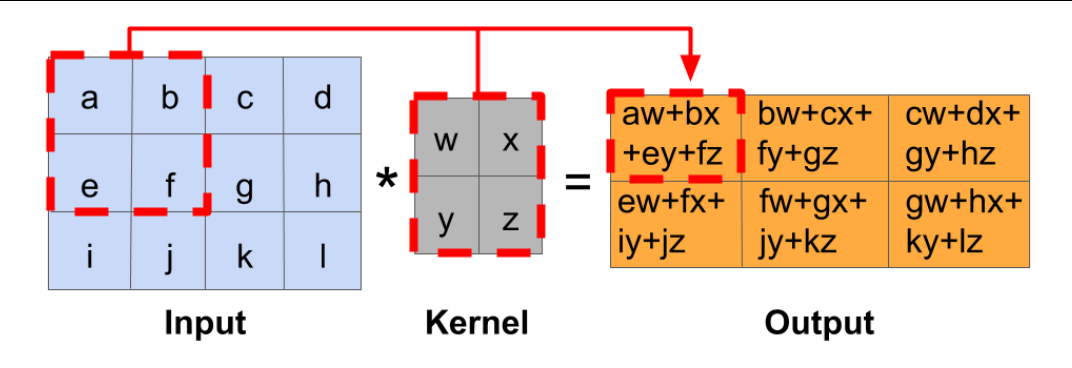
\includegraphics[width=0.7\textwidth]{images/arte/cnn1}
	\caption{Ejemplo de una convolución de dos dimensiones. Fuente \cite{temariodeeplearning}}
	\label{fig:cnn1}
\end{figure}


TODO Reduccion dimensión padding...

El proceso explicado anteriormente correspondería con una capa convolucional, que son el corazón de las redes neuronales convolucionales, sin embargo, en una red neuronal convolucional estas capas coexisten con otro tipo de capas que nos ayudaran a mejorar nuestros modelos. Las más usuales son:

\begin{itemize}
	\item Capa de agrupamiento (\textit{polling} en inglés): El objetivo de esta capa es agrupar un conjunto de salidas para obtener un único valor, al conjunto de valores de entrada (seleccionado de nuevo con un filtro) se le aplica una función para obtener un único valor. Aunque se pueden utilizar diferentes funciones, como puede ser la media, lo más usual es aplicar la función de máximo (\textit{max-polling}). Es habitual, intuir que usando esta función nos estamos quedando con las características más relevantes de cada cuadrante (del tamaño del filtro) de la entrada.
	\item Capa totalmente conectada: Hemos visto ejemplos de capas totalmente conectada al introducir las redes neuronales, esta capas usualmente se usan al final de nuestra red para tareas de clasificación, teniendo la última capa un número de neuronas igual al número de clases que pretendemos clasificar.
	\item Capa RELU: Si observamos la descripción de la operación de convolución nos damos cuenta de que se trata de una operación totalmente lineal, es por ello que después de cada capa de convolución es usual agregar una capa no lineal (también llamada capa de activación). Aunque se pueden utilizar otras funciones como la tangente o la función sigmoide, lo más usual es utilizar la función RELU.
	
	\item Capa de Dropout: 
	
\end{itemize}

En una red neuronal convolucional normalmente coexisten otro tipo de



TODO seguir con pooling ...

Encontramos una explicación más profunda sobre las redes convolucionales y su uso general en \cite{temariodeeplearning}. Nosotros nos centraremos en tener una visión general de su aplicación al Procesamiento del Lenguaje Natural, que también puede ampliarse en \cite{goldberg_2017}.


TODO palabras

\subsubsection{Redes neuronales recurrentes}


TODO explicación pros y contras

\section{BigData y Fast Data}

El primer uso del término  \textit{Big Data}  se da en un artículo de Michael Cox y David Ellsworth de la NASA publicado en 1997 (\cite{Cox_1997}), donde hacen referencia a la dificultad de procesar grandes volúmenes de datos con los métodos de la época. Sin embargo, fue en 2001 cuando encontramos la definición más conocida y aceptada de \textit{Big Data} hecha por el analista Laney Douglas en su artículo ``3D Data Management: Controlling Data Volume, Velocity y Variety''(\cite{laneay_2013}) en el que se hacía referencia a las ya ``famosas'' tres \textit{V}s:

\begin{itemize}
	\item \textbf{V}olumen:  Cada vez los volúmenes de datos son mayores.
	\item \textbf{V}elocidad: Es cada vez mayor la velocidad con la que se generan los datos.  
	\item \textbf{V}ariedad: Dejamos de tener únicamente datos completamente estructurados para trabajar con datos no estructurados y/o  semi-estructurados. 
\end{itemize} 


Google, como es obvio, también  se enfrentó a un importante problema a la hora de procesar la ingente cantidad de datos que generaba día a día y que no podían ser procesados de manera eficiente con el \textit{software} existente, es por ello que en el año 2003 presenta en \cite{GFS} su  \textit{``Google File System''} (GFS) y un año después \textit{Map Reduce} \cite{MapReduce}, estas dos capas de almacenamiento y procesamiento distribuido dieron lugar al nacimiento de lo que hoy conocemos como \textit{\textbf{Big Data}}.

Sin embargo, estas aportaciones no empezaron a tomar una repercusión relevante fuera de Google hasta el nacimiento del \textit{framework} Hadoop en 2006, un ecosistema con una gran cantidad de servicios pero cuya base fue Map Reduce y HDFS (basado en GFS). La complejidad del ecosistema \textit{Hadoop} hizo que éste no empezara a aparecer en las mayoría de las empresas hasta la creación de la compañía \textit{Cloudera} en 2009, que empezó a empaquetar los diferentes componentes del ecosistema \textit{Hadoop}, ofreciendo distribuciones estables y soporte para sus clientes. 

Durante estos 10 años la popularidad de \textit{Hadoop} ha crecido exponencialmente y junto con las BBDD NoSQL, nacidas también a partir de Google con su BigTable, forman lo que hoy conocemos como Big Data. 



El auge del \textbf{Big Data} ha llevado a algunas empresas a tener verdadera obsesión por el almacenamiento de todos los datos de sus clientes y las operaciones realizadas, creando inmensos \textit{datalakes} donde tener enormes históricos de todos sus datos, este ``síndrome de Diógenes digital'' creado por falsas expectativas, por la imposibilidad de extraer valor de los datos o por la dimensión cambiante de las empresas actuales, en la que los datos de años atrás pueden no ser relevantes en el presente, es uno de los posibles motivos por lo que el tratamiento de los datos esta cambiando. Otro de los motivos para el cambio de rumbo del \textit{Big Data} está relacionado con la \textit{V} de Velocidad, hoy en día no solo es importante la capacidad de ingestar rápidamente los datos, sino la capacidad de poder procesar y obtener decisiones o actuar en tiempo real a partir de los datos, aportando valor al negocio. En este escenario se vuelve más importante la velocidad que el volumen de datos, esto es lo que se denomina \textit{Fast Data}. 

Dentro del \textit{Fast Data} es habitual el uso de BBDD \textit{in-memory}, de buses de eventos y de tecnologías de procesamiento capaces de procesar los eventos en tiempo real. Como veremos posteriormente al desarrollar nuestra arquitectura, el \textit{Fast Data} será una parte fundamental en nuestro proyecto en el que tendremos que clasificar las llamadas en tiempo real y tomar decisiones (o alarmar) en función de las mismas.
